\chapter{Numerical Results}

In this chapter the main calculations of the proposed theories and will be presented. 

\section{Verification}

\section{Validation}
For verification purposes the numerical benchmark presented in \cite{Hron2006} has been chosen for this thesis. This benchmark as been widely accepted throughout the fluid-structure interaction community as a rigidly validation benchmark. This is mainly due to its diversity of tests included, challenging all the main components of a FSI solver. \\
The benchmark is divided into three main testenvironments.
In the first environment the purely fluid solver is tested for a range of different inflow parameters. \\
The second environment regards the purely structure implementation, regarding bending of the elastic flag. We will in this thesis consider the final environment, testing the total system in terms of a fluid-structure interaction problem. The others have been tested and proved to be an essential part of the development of the solver, but will for brevity not be reported. \\ \\

The fluid-structure interaction validation benchmark is divided into three different problems with increasing difficulty, posing different challenges to the implementation. 
Each problem alters the fluid and solid parameters to provoke different behavior of the system.

\begin{figure}
  \caption{Domain configuration}
  \centering
    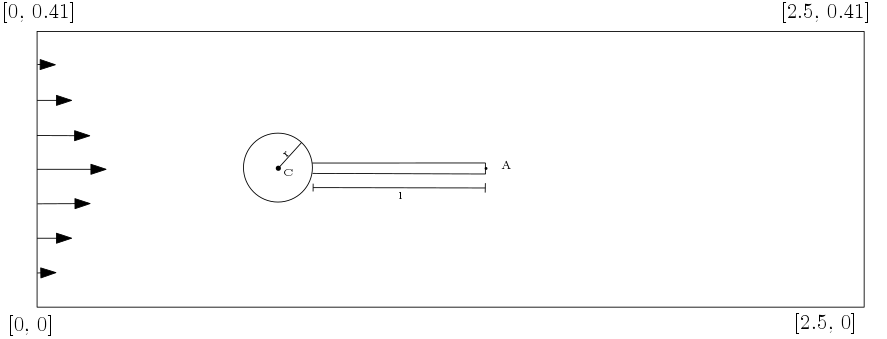
\includegraphics[scale=0.5]{./Fig/turekflag.png}
\end{figure}

Several quantites for comparion is presented in \cite{Hron2006} for validation purposes. We will report
\begin{itemize}
\item The position of point A(t) as the strucutre undergoes deformation.
\item Drag and lift forces exerted on of the whole interior geometry in contact with the fluid, consisting of the rigid circle and the elastic beam. 
\begin{align*}
(F_D, F_L) = \int_{\Gamma} \mathbf{\sigma} \cdot \mathbf{n} dS
\end{align*}
Where \textbf{n} is the unit normal vector, pointing into the fluid domain. 
\end{itemize}
The amplitude and mean values for the time dependent properties are calculated from the last period of oscillations, together with the period. 

\begin{table}[h]
\centering
\caption{Benchmark environment}
\label{my-label}
\begin{tabular}{ |p{3cm}||p{3cm}|p{3cm}|p{3cm}|  }
 \hline
 \multicolumn{4}{|c|}{Solid parameters} \\
 \hline
 parameter              & FSI1 & FSI2 & FSI3 \\
 \hline
 $\rho^s [10^{3} \frac{kg}{m^3}]$ & 1    & 10   & 1    \\
$\nu^s$ & 0.4  & 0.4  & 0.4  \\
$\mu^s  [10^{6}\frac{kg}{ms^2}]$  & 0.5  & 0.5  & 2.0  \\
 \hline
 \multicolumn{4}{|c|}{Fluid parameters} \\
 \hline
$\rho^f [10^{3}\frac{kg}{m^3}]$ & 1    & 1    & 1    \\
$\nu^f  [10^{-3}\frac{m^2}{s}]$  & 1    & 1    & 1    \\
U                      & 0.2  & 1    & 2    \\
parameter              & FSI1 & FSI2 & FSI3 \\
Re                     & 20   & 100  & 200 \\
\hline
\end{tabular}
\end{table}


\subsection{FSI1}
The first environment yields a steady state solution for the system. It is meant as a basic implementation test as it applies small deformations to the system. Therefore is provides a test for the solving procedure, but doesn't excess large constrain of choice of mesh extrapolation operator. 

\begin{table}[h!]
\centering
\caption{FSI 1}
\label{my-label}
\begin{tabular}{ |p{2.5cm}||p{1cm}|p{1cm}|p{2.3cm}|p{2.3cm}|p{1.2cm}|p{1.2cm}|}
 \hline
  \multicolumn{7}{|c|}{$\Delta t = 0.5$} \\
   \hline
 Model & nel & ndof & ux of A [x $10^{3}$]  &uy of A [x $10^{3}$]& Drag  & Lift \\
 \hline
Biharmonic bc2 & 1 &1 & 0.0228  &  0.7740  & 14.17280  &  0.7614 \\
 \hline
Biharmonic bc1 & 1 &1 & 0.0228 &   0.7737  & 14.17281 &  0.7612  \\
 \hline
Elastic        & 1 &1 & 0.0227  &  0.7960  & 14.17283 &  0.7607  \\
 \hline
Laplace        & 1 &1 & 0.0227  &  0.7958  & 14.17285 &  0.7607   \\
 \hline
  \multicolumn{7}{|c|}{$\Delta t = 0.1$} \\
   \hline
 Model & nel & ndof & ux of A [x $10^{3}$]  &uy of A [x $10^{3}$]& Drag  & Lift \\
 \hline
Biharmonic bc2 & 1 &1 & 0.0228 &  0.7743  & 14.17279 & 0.76162  \\
 \hline
Biharmonic bc1 & 1 &1 & 0.0228  &  0.7739 & 14.17280 & 0.76142 \\
 \hline
Elastic       & 1 &1 & 0.0228  &  0.7962  & 14.17281 & 0.76092 \\
 \hline
Laplace        & 1 &1 & 0.0228  & 0.7961  & 14.17284 & 0.76090 \\
\hline
\end{tabular}
\end{table}

\subsection{FSI2}
The second environment results in a periodic solution. It proved to be one of the most demanding tests due to its large deformation, leading to the risk of entangled mesh cells. As such this raised the need for a high quality extrapolation of the solid deformation.
\\
\subsection{FSI3}    
The final environment does not induce deformation to the extent of the FSI2 benchmark. However a critical phase in the transition to the periodic solution was discovered, where the pressure oscillation induces a large deformation to the system. 

\begin{table}[h!]
\centering
\caption{FSI 3}
\label{my-label}
\begin{tabular}{lllll}
 \hline
Test & x-comp A          & y-comp A             & drag                   & lift                 \\
 \hline
bc1 &                   &                      & 442.9 +/ 17.26         & 2.83 +- 148.8        \\
 \hline
bc2 &                   &                      & 442.8 +/ 17.44         & 3.06 +-147.9         \\
 \hline
Ref & 2.69  2.53  &   1.48  34.38 5.3   & 457. 22.66 10.9 & 2.22 149.78 5.3 \\
 \hline
\end{tabular}
\end{table}


\section{Mesh movement}
The final enviroment 